% !TEX TS-program = xelatex

% Copyright 2010 by Pedro Furlanetto 
%
% In principle, this file can be redistributed and/or modified under
% the terms of the GNU Public License, version 2.

% Based on Till Tantau beamer template

\documentclass{beamer}
%\documentclass[draft]{beamer}

\mode<presentation>
{
  \usetheme{Warsaw}
  \setbeamercovered{transparent}
}


\usepackage{hyperref}
\usepackage{graphicx}
\usepackage[english]{babel}
%\usepackage[utf8]{inputenc}
\usepackage{times}
\usepackage[T1]{fontenc}
\usepackage{xltxtra} % Extra customizations for XeLaTeX
\usepackage{color}
\usepackage{listings}
 

% "define" Scala
\lstdefinelanguage{Scala}{
  morekeywords={abstract,case,catch,class,def,%
    do,else,extends,false,final,finally,%
    for,if,implicit,import,match,mixin,%
    new,null,object,override,package,%
    private,protected,requires,return,sealed,%
    super,this,throw,trait,true,try,%
    type,val,var,while,with,yield}, % scala>
  otherkeywords={=>,<-,<\%,<:,>:,\#,@,=,:},
  sensitive=true,
  morecomment=[l]{//},
  morecomment=[n]{/*}{*/},
  morestring=[b]",
  morestring=[b]',
  morestring=[b]""",
  literate={=>}{$\Rightarrow$ }2 {<-}{$\leftarrow$}2 {->}{$\rightarrow$}2
}


\definecolor{dkgreen}{rgb}{0,0.6,0}
\definecolor{gray}{rgb}{0.5,0.5,0.5}
\definecolor{mauve}{rgb}{0.58,0,0.82}

% Default settings for code listings
\lstset{frame=tb,
  language=Scala,
  aboveskip=3mm,
  belowskip=3mm,
  showstringspaces=false,
  columns=flexible,
  basicstyle={\scriptsize\ttfamily},
  numbers=none,
  numberstyle=\tiny\color{gray},
  keywordstyle=\color{blue},
  commentstyle=\color{dkgreen},
  stringstyle=\color{mauve},
  frame=single,
  breaklines=true,
  breakatwhitespace=true,
  tabsize=3,
  mathescape=true,
  resetmargins=true,
  showtabs=true
}

\setbeamertemplate{navigation symbols}{}%remove navigation symbols

\title{Scala Relâmpago}

\subtitle{Preciso de um subtítulo descritivo}

\author{Pedro Furlanetto}

\institute
{
  Ideais Tecnologia\\
\begin{minipage}{0.6\textwidth}
\begin{flushleft} 

\includegraphics[height=1.5cm]{ideaisconf.png} 
\end{flushleft}
\end{minipage}
\begin{minipage}{0.3\textwidth}
\centering{ 
\includegraphics[height=2cm]{ideais-grande.jpg}}
\end{minipage}
  
}

\date[IC 2010] % (optional, should be abbreviation of conference name)
{IdeaisConf, 2010}

\subject{Linguagem de Programação Scala}

%\logo{
\includegraphics[height=1cm]{ideais-grande.jpg}}

\AtBeginSubsection[]
{
  \begin{frame}<beamer>{Resumo}
    \tableofcontents[currentsection,currentsubsection,sectionstyle=show/shaded,subsectionstyle=show/shaded/shaded]
  \end{frame}
}

%\beamerdefaultoverlayspecification{<+->}

\begin{document}

\begin{frame}  
  \centering{
\includegraphics[height=1cm]{Scala_Logo2008.png}}
  \titlepage
\end{frame}

%\begin{frame}{Resumo}
%  \tableofcontents
%\end{frame}

\section{Overview}

\subsection{De onde veio}

\begin{frame}{Criada por} 
	\begin{itemize}
	\item Martin Odersky - \emph{École Polytechnique Fédérale de Lausanne} (EPFL), Lausanne, Switzerland em 2001
	\begin{itemize}
	   \item Ph.D. com \emph{Niklaus Wirth} (criador do Pascal)
              \item \emph{GJ} e \emph{Pizza} com \emph{Philip Wadler} - deu origem ao \emph{generics} do Java atual
	\end{itemize}	
	\end{itemize}
           \begin{columns}
           \begin{column}{.5\textwidth}
               \centering{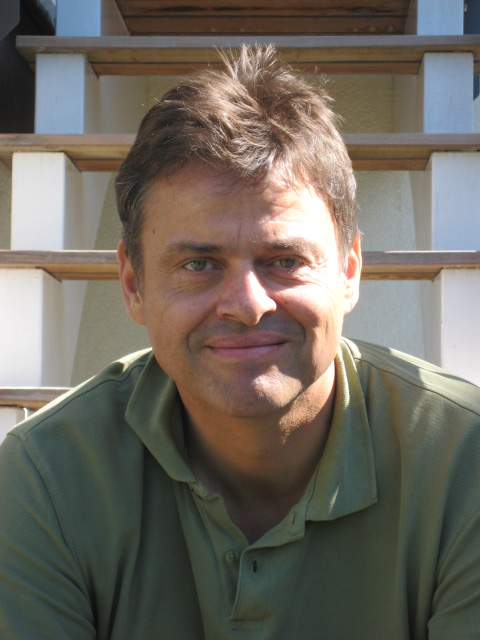
\includegraphics[height=4cm]{Martin-Odersky.jpg}}
           \end{column}
           \begin{column}{.5\textwidth}
               \centering{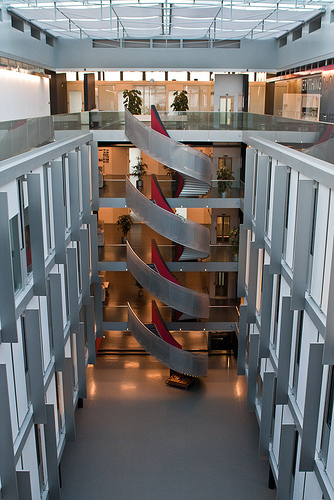
\includegraphics[height=4cm]{scala-the-real-thing.jpg}}
           \end{column}
	\end{columns}
\end{frame}

\subsection{O que é Scala?}

\begin{frame}{Unifica funcional e orientação a objeto} 
    \centering{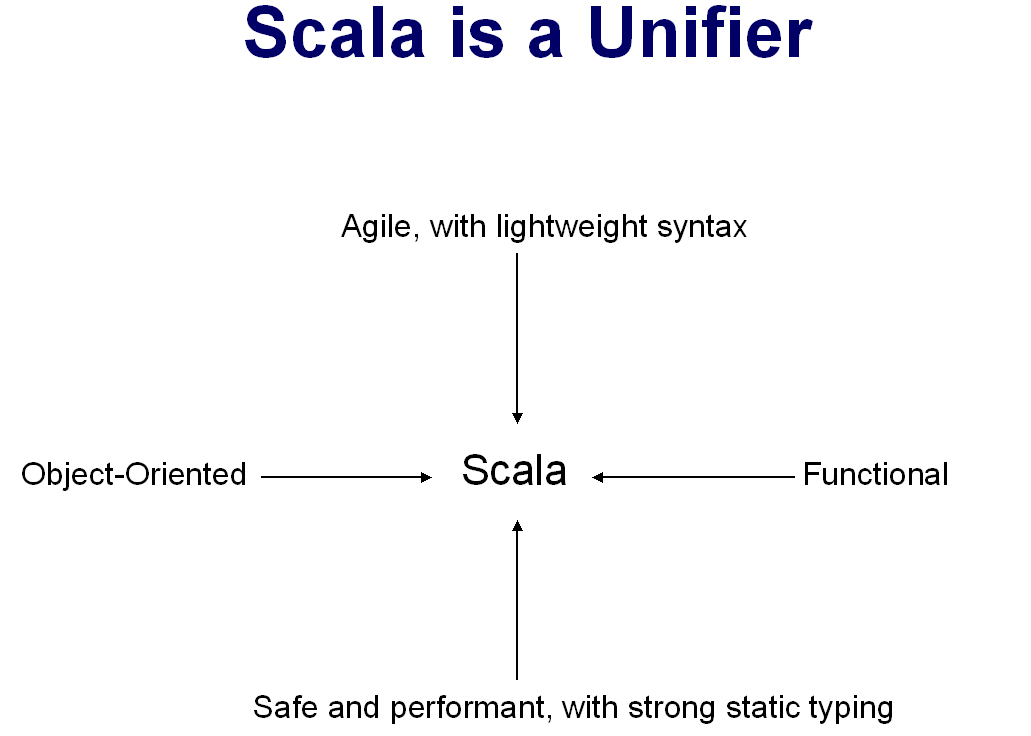
\includegraphics[scale=0.20]{Scala-is-a-Unifier.png}} 
\end{frame}

\begin{frame}[fragile]{Algumas características} 
    \begin{itemize} %[<+->]
        \item Sintaxe simples e consistente 
        \begin{itemize}
              \item Exemplo: imports em qualquer lugar limitados pelo escopo 
        \end{itemize}
        \item Baseado em expressões
        \item Tudo são objetos e chamadas de métodos (ala \emph{Smalltalk})
	\begin{lstlisting}
		1 + 5 * 4 == 1.+(5.*(4))
	 \end{lstlisting}
        \item Inferência de tipos
        \item Closures e funções como \emph{first-class citizens}
	\begin{lstlisting}
	scala> val string2int = (s:String) => Integer.parseInt(s)	
	string2int: (String) => Int = <function1>
	scala> string2int("5")
	res26: Int = 5
	\end{lstlisting}
         \item Herança múltipla com \emph{traits e mixins}
    \end{itemize}
\end{frame}

\begin{frame}[fragile]{Mais algumas características} 
    \begin{itemize} %[<+->]
        \item Linha de comando - \emph{REPL}
        \item Accessors e Mutators automáticos
        \item Construtor e propriedades juntos
        \item Argumentos defaults e nomeados
		\begin{lstlisting}
		scala> class Exemplo(var nome:String = "<Sem Nome>", 
			var idade:Int = 18)
		scala> val e = new Exemplo()
		scala> (e.idade, e.nome)
		res6: $\textbf{(Int, String) = (18,<Sem Nome>)}$
		scala> val e2= new Exemplo(idade = 20)
		scala> (e2.idade, e2.nome)
		res9: $\textbf{(Int, String) = (20,<Sem Nome>)}$
		\end{lstlisting}
    \end{itemize}
\end{frame}

\begin{frame}[fragile]{Mais algumas características} 
    \begin{itemize} %[<+->]
        \item Scala não tem \emph{métodos estáticos} - mas tem \emph{objetos companheiros}
        \begin{itemize}
	\item Uma declaração \emph{object} no mesmo fonte e com o mesmo nome da classe
        \end{itemize}
        \item \emph{Case Classes}
        \begin{itemize}
              \item Uma classe que já implementa \emph{hashCode}, \emph{equals}, \emph{clone} e \emph{toString} 
	   \item Também implementa um \emph{objeto companheiro} com os métodos \emph{apply} e \emph{unapply}
        \end{itemize}
        \item Método \emph{apply} funciona como um ``método default''
        \item Método \emph{unpply} serve para ``desconstruir'' uma classe
    \end{itemize}
\end{frame}

\begin{frame}[fragile]{Mais algumas características} 
    \begin{itemize} %[<+->]
        \item Refazendo o exemplo como \emph{Case Classe} e um \emph{objeto companheiro}
	\begin{lstlisting}
	case class Exemplo(var nome:String = "<Sem Nome>", 
		var idade:Int = 18); 
	object Exemplo {
	  def media(e:Exemplo, e2:Exemplo) =
	     ( e.idade + e2.idade ) / 2
	}
	> val e = Exemplo(idade=20, nome="Fulano")
	e: Exemplo = $\textbf{Exemplo(Fulano,20)}$
	> val e2 = Exemplo("João",30)
	e2: Exemplo = $\textbf{Exemplo(João,30)}$
	> Exemplo.media(e,e2)
	res10: Int = $\textbf{25}$
	\end{lstlisting}
    \end{itemize}
\end{frame}

\begin{frame}[fragile]{\emph{for-comprehensions}} 
    \begin{itemize} %[<+->]
    \item Andar, filtrar e colher dados de listas com facilidade
	\begin{lstlisting}
	> val E = Exemplo.apply _
	E: (String, Int) => Exemplo = <function2>
	
> val lista = List(E("Roberto",34), E("Maria",15), E("João",18), E("Rosa",21), E("Fulana",8), E("Fulano",5), E("Ivo",30), E("Joana",10),E("Igor",18), E("Gustavo",21))
	
	> val maiores = for(e <- lista; if e.idade >= 18 ) yield e
	maiores: List[Exemplo] = List(Exemplo(Roberto,34), Exemplo(João,18), Exemplo(Rosa,21), Exemplo(Ivo,30), Exemplo(Igor,18), Exemplo(Gustavo,21))	
	\end{lstlisting}
    \end{itemize}
\end{frame}

\begin{frame}[fragile]{\emph{for-comprehensions}} 
    \begin{itemize} %[<+->]
	\item Andar, filtrar e colher dados de listas com facilidade
	\item<1-> Agora todos que tem a mesma idade, mas sem repetir
	\begin{lstlisting}
	> val mesmaIdade = for(
	      (e1, idx) <- lista.zipWithIndex
	             e2 <- lista.drop(idx + 1)
	      if e1 != e2 && e1.idade == e2.idade) 
	          yield  (e1, e2)
	mesmaIdade: List[(Exemplo, Exemplo)] = List((Exemplo(João,18),Exemplo(Igor,18)), (Exemplo(Rosa,21),Exemplo(Gustavo,21)))
	\end{lstlisting}

	\item \textbf{Calma!} Não é tão complicado.
	\begin{lstlisting}
	> lista.zipWithIndex.take(4)
	List[(Exemplo, Int)] = List((Exemplo(Roberto,34),0), (Exemplo(Maria,15),1), (Exemplo(João,18),2), (Exemplo(Rosa,21),3))
	\end{lstlisting}
    \end{itemize}
\end{frame}

\begin{frame}[fragile]{\emph{Pattern Matches}} 
    \begin{itemize} %[<+->]
	\item ``Descontruir'' objetos com facilidade
	\begin{lstlisting}	
	> lista(0)
	Exemplo = Exemplo(Roberto,34)
	
	> val Exemplo(nome,idade) = lista(0)
	nome: String = Roberto
	idade: Int = 34
	\end{lstlisting}
	
	\item Ou só uma parte do objeto
	\begin{lstlisting}	
	> lista.collect { case Exemplo(nome,18) => nome }
	List[String] = List(João, Igor)	
	\end{lstlisting}
    \end{itemize}
\end{frame}


\section{Ainda tem muito mais}

\subsection{O que não vimos?}

\begin{frame}{O que não vimos?}
	\begin{itemize} %[<+->]
	\item \emph{Traits} e \emph{Mixins} - Herança multipla controlada
	\item \emph{Parâmetros Implicitos} - ``Injeção de dependencia transparente?''
	\item \emph{Pimp-my-libray} - adicionando métodos a classes já existentes
	\item \emph{Self-types} - Representando dependencias entre classes e traits 
	\item \emph{Tipos estruturais} - a.k.a. \emph{Duck typing done right}
	\item \emph{Option objects} - null object
	\item \emph{Parâmetros por nome} - ``avaliação tardia''
	\end{itemize}
\end{frame}

\subsection{Será que é complicado?}

\begin{frame}{Será que é complicado?}
	\begin{columns}
           \begin{column}{.5\textwidth}               
              \centering{``\emph{Com grandes poderes vêm grandes responsabilidades.}''}
           \end{column}
           \begin{column}{.5\textwidth}
               
\includegraphics[height=5cm]{spiderman.png}
           \end{column}
	\end{columns}	
\end{frame}

\section{Referências}

\begin{frame}{Para aprender mais}
	\begin{itemize} 
	\item \url{http://www.scala-lang.org}
		\begin{itemize} 
			\item A Tour of Scala
			\item Scala by Example
			\item A Brief Scala Tutorial
		\end{itemize}
	\item \url{http://planetscala.org} - agregador de blogs sobre Scala
	\item Programming Scala 
	\end{itemize}
\end{frame}



\end{document}


